%!TeX encoding = UTF-8
%!TeX program = xelatex
\documentclass[notheorems, aspectratio=54]{beamer}
% aspectratio: 1610, 149, 54, 43(default), 32

\usepackage{latexsym}
\usepackage{amsmath,amssymb}
\usepackage{mathtools}
\usepackage{color,xcolor}
\usepackage{graphicx}
\usepackage{algorithm}
\usepackage{amsthm}
\DeclareMathOperator*{\argmax}{argmax} % thin space, limits underneath in displays
\usepackage{lmodern} % 解决 font warning
% \usepackage[UTF8]{ctex}
\usepackage{animate} % insert gif

\usepackage{lipsum} % To generate test text 
\usepackage{ulem} % 下划线,波浪线

\usepackage{listings} % display code on slides; don't forget [fragile] option after \begin{frame}

% ----------------------------------------------
% tikx
\usepackage{framed}
\usepackage{fancybox}
\usepackage{tikz}
\usepackage{tikz-qtree}
\usepackage{pgf}
\usetikzlibrary{automata, calc,trees,positioning,arrows,chains,shapes.geometric,%
    decorations.pathreplacing,decorations.pathmorphing,shapes,%
    matrix,shapes.symbols}
\pgfmathsetseed{1} % To have predictable results
% Define a background layer, in which the parchment shape is drawn
\pgfdeclarelayer{background}
\pgfsetlayers{background,main}

% define styles for the normal border and the torn border
\tikzset{
  normal border/.style={orange!30!black!10, decorate, 
     decoration={random steps, segment length=2.5cm, amplitude=.7mm}},
  torn border/.style={orange!30!black!5, decorate, 
     decoration={random steps, segment length=.5cm, amplitude=1.7mm}}}

% Macro to draw the shape behind the text, when it fits completly in the
% page
\def\parchmentframe#1{
\tikz{
  \node[inner sep=2em] (A) {#1};  % Draw the text of the node
  \begin{pgfonlayer}{background}  % Draw the shape behind
  \fill[normal border] 
        (A.south east) -- (A.south west) -- 
        (A.north west) -- (A.north east) -- cycle;
  \end{pgfonlayer}}}

% Macro to draw the shape, when the text will continue in next page
\def\parchmentframetop#1{
\tikz{
  \node[inner sep=2em] (A) {#1};    % Draw the text of the node
  \begin{pgfonlayer}{background}    
  \fill[normal border]              % Draw the ``complete shape'' behind
        (A.south east) -- (A.south west) -- 
        (A.north west) -- (A.north east) -- cycle;
  \fill[torn border]                % Add the torn lower border
        ($(A.south east)-(0,.2)$) -- ($(A.south west)-(0,.2)$) -- 
        ($(A.south west)+(0,.2)$) -- ($(A.south east)+(0,.2)$) -- cycle;
  \end{pgfonlayer}}}

% Macro to draw the shape, when the text continues from previous page
\def\parchmentframebottom#1{
\tikz{
  \node[inner sep=2em] (A) {#1};   % Draw the text of the node
  \begin{pgfonlayer}{background}   
  \fill[normal border]             % Draw the ``complete shape'' behind
        (A.south east) -- (A.south west) -- 
        (A.north west) -- (A.north east) -- cycle;
  \fill[torn border]               % Add the torn upper border
        ($(A.north east)-(0,.2)$) -- ($(A.north west)-(0,.2)$) -- 
        ($(A.north west)+(0,.2)$) -- ($(A.north east)+(0,.2)$) -- cycle;
  \end{pgfonlayer}}}

% Macro to draw the shape, when both the text continues from previous page
% and it will continue in next page
\def\parchmentframemiddle#1{
\tikz{
  \node[inner sep=2em] (A) {#1};   % Draw the text of the node
  \begin{pgfonlayer}{background}   
  \fill[normal border]             % Draw the ``complete shape'' behind
        (A.south east) -- (A.south west) -- 
        (A.north west) -- (A.north east) -- cycle;
  \fill[torn border]               % Add the torn lower border
        ($(A.south east)-(0,.2)$) -- ($(A.south west)-(0,.2)$) -- 
        ($(A.south west)+(0,.2)$) -- ($(A.south east)+(0,.2)$) -- cycle;
  \fill[torn border]               % Add the torn upper border
        ($(A.north east)-(0,.2)$) -- ($(A.north west)-(0,.2)$) -- 
        ($(A.north west)+(0,.2)$) -- ($(A.north east)+(0,.2)$) -- cycle;
  \end{pgfonlayer}}}

% Define the environment which puts the frame
% In this case, the environment also accepts an argument with an optional
% title (which defaults to ``Example'', which is typeset in a box overlaid
% on the top border
\newenvironment{parchment}[1][Example]{%
  \def\FrameCommand{\parchmentframe}%
  \def\FirstFrameCommand{\parchmentframetop}%
  \def\LastFrameCommand{\parchmentframebottom}%
  \def\MidFrameCommand{\parchmentframemiddle}%
  \vskip\baselineskip
  \MakeFramed {\FrameRestore}
  \noindent\tikz\node[inner sep=1ex, draw=black!20,fill=white, 
          anchor=west, overlay] at (0em, 2em) {\sffamily#1};\par}%
{\endMakeFramed}

% ----------------------------------------------

\mode<presentation>{
    \usetheme{CambridgeUS}
    % Boadilla CambridgeUS
    % default Antibes Berlin Copenhagen
    % Madrid Montpelier Ilmenau Malmoe
    % Berkeley Singapore Warsaw
    \usecolortheme{beaver}
    % beetle, beaver, orchid, whale, dolphin
    \useoutertheme{infolines}
    % infolines miniframes shadow sidebar smoothbars smoothtree split tree
    \useinnertheme{circles}
    % circles, rectanges, rounded, inmargin
}
% 设置 block 颜色
\setbeamercolor{block title}{bg=red!30,fg=white}

\newcommand{\reditem}[1]{\setbeamercolor{item}{fg=red}\item #1}

% 缩放公式大小
\newcommand*{\Scale}[2][4]{\scalebox{#1}{\ensuremath{#2}}}

% 解决 font warning
\renewcommand\textbullet{\ensuremath{\bullet}}

% ---------------------------------------------------------------------
% flow chart
\tikzset{
    >=stealth',
    punktchain/.style={
        rectangle, 
        rounded corners, 
        % fill=black!10,
        draw=white, very thick,
        text width=6em,
        minimum height=2em, 
        text centered, 
        on chain
    },
    largepunktchain/.style={
        rectangle,
        rounded corners,
        draw=white, very thick,
        text width=10em,
        minimum height=2em,
        on chain
    },
    line/.style={draw, thick, <-},
    element/.style={
        tape,
        top color=white,
        bottom color=blue!50!black!60!,
        minimum width=6em,
        draw=blue!40!black!90, very thick,
        text width=6em, 
        minimum height=2em, 
        text centered, 
        on chain
    },
    every join/.style={->, thick,shorten >=1pt},
    decoration={brace},
    tuborg/.style={decorate},
    tubnode/.style={midway, right=2pt},
    font={\fontsize{10pt}{12}\selectfont},
}
% ---------------------------------------------------------------------

% code setting
\lstset{
    language=C++,
    basicstyle=\ttfamily\footnotesize,
    keywordstyle=\color{red},
    breaklines=true,
    xleftmargin=2em,
    numbers=left,
    numberstyle=\color[RGB]{222,155,81},
    frame=leftline,
    tabsize=4,
    breakatwhitespace=false,
    showspaces=false,               
    showstringspaces=false,
    showtabs=false,
    morekeywords={Str, Num, List},
}

% ---------------------------------------------------------------------

%% preamble
\title{Lecture 07}
% \subtitle{The subtitle}
\author{Dihui Lai}
\institute[WUSTL]{dlai@wustl.edu}

% -------------------------------------------------------------

\begin{document}

%% title frame
\begin{frame}
    \titlepage
\end{frame}


\begin{frame}
CONTENT
\begin{itemize}
\item Supervised Learning v.s. Unsupervised Learning
\item CART (Classification and Regression Tree)
\item Random Forest
\item Gradient Boosting Trees
\end{itemize} 
\end{frame}


%% normal frame
\section{Supervised Learning v.s. Unsupervised Learning}

\begin{frame}
\frametitle{Supervised Learning v.s. Unsupervised Learning}
\begin{itemize}
\item \textbf{Supervised Leaning}: a model/algorithm that is built on a dataset that contains both input data and desired outcome. For example, logistic regression; linear regression.
\item \textbf{Unsupervised Leaning}: a model/algorithm that is built on a dataset that contains both input data but no desired outcome. For example, K-mean clustering
\end{itemize}
\end{frame}

%% normal frame
\section{CART}
\begin{frame}
    \frametitle{CART: Impurity Measurement}
    At node $\mathnormal{t}$, the fraction of class $\mathnormal{i}$ is denoted as $\mathnormal{p(i|t)}$
    
    Entropy: $\mathnormal{H(t)=-\sum\limits_{i=1}^{C}p(i|t)\log(p(i|t))}$
    
    Gini-Index: $\mathnormal{Gini(t)=\sum\limits_{i=1}^{C}[p(i|t)]^2}$
    
    Classification Error: $\mathnormal{Error(t)=1-\max\limits_{i}p(i| t)}$
\end{frame}

\begin{frame}
    \frametitle{Entropy}
    Considering the entropy of a data set that contains two types of outcomes: {0, 1}. Running 10 experiments, we get the following out comes (0, 0, 1, 0, 1, 0, 1, 1, 0, 1). The entropy is 
    $$
    \mathnormal{ H(t)}=-\sum\limits_{i=1}^{2}\frac{1}{2}\log_2(\frac{1}{2})=1
    $$
    
What if we have out come of (1, 1, 1, 1, 1, 1, 1, 1, 1, 1)? The entropy is 
    $$
    \mathnormal{H(t)}=1\log_2(1)+0\log_2(0)=0
    $$

The less variance in the data, the smaller the entropy is. For binary outcome, a probability of 1/2 leads to the largest uncertainty/entropy.

\end{frame}

\begin{frame}
\frametitle{CART Model}
John likes playing tennis on Saturday, The liklihood of John playing tennis depends on the weather. John has never played on a rainy. He may or may not play on a windy day. Given the weather, can you predict if John will play tennis this weekend?

\begin{center}
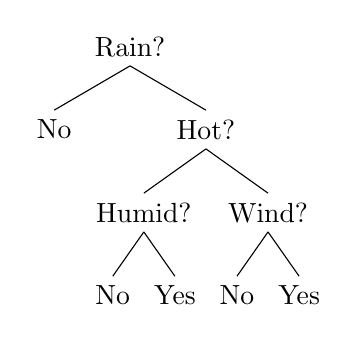
\begin{tikzpicture}
\tikzset{every tree node/.style={align=center,anchor=north}}
\Tree [.Rain? No 
		[.Hot? [.Humid? No Yes ][.Wind? No Yes ] ] ]
\end{tikzpicture}
\end{center}
\end{frame}

\begin{frame}
\frametitle{CART Model: How to Grow a Tree?}
\begin{itemize}
\item At each node, the tree algorithm will check every variable for a possible split. 
\item A variable is selected for the split if it maximally reduces the impurity in the child nodes (e.g. the largest reduction of entroy, the largest reduction of variance etc.)
\item Pruning: a tree can grow till each leave only contains one data point. Pruning the tree is needed to avoid overfitting.
\end{itemize}
\end{frame}

\begin{frame}
\frametitle{CART Model: Stopping Criterion}
Stopping criterion
\begin{itemize}
\item[-] The number of training sample after split is less than certain number 'min\_ samples\_ split'.
\item[-] When the depth of the tree reaches to certain threshold 'max\_ depth'.
\end{itemize}
\end{frame}

\begin{frame}
\frametitle{Information Gain at a Split Node}
Assuming we collect John's tennis activities for 20 weeks. Out of the 20 weekends, we have 8 sunny day and John plays tennis on all of them. Out of the rest 12 days, John played tennis on 7 days. 
Before any split, we have the entropy calculated as 
    $$
     \mathnormal{H(root)}=-\frac{15}{20}\log(\frac{15}{20})-\frac{5}{20}\log(\frac{5}{20})=0.562
    $$
Split based on the weather, we have on sunny days
$
 \mathnormal{H(sunny)=0}
$
and on other days
$
\mathnormal{H(!sunny)}=-\frac{7}{12}\log(\frac{7}{12})-\frac{5}{12}\log(\frac{5}{12})=0.679
$
Therefore the child nodes have average entropy of 
$$
\mathnormal{H(childs)}=\frac{8}{20}\cdot 0+\frac{12}{20}\cdot 0.679=0.407
$$
We have entropy reduced by $\mathnormal{\Delta H}=0.562-0.390=0.154$
\end{frame}

\begin{frame}
\frametitle{Information Gain at a Split Node}
Instead of splitting by forcast, we look at the wind speed. Out of the 20 weekends, 10 days are windy and 10 days are not windy. Out of the windy day, John played 6 times and 9 times for the non-windy days.

Split based on the wind condition, we have on windy days
$
\mathnormal{H(!windy)}=-\frac{6}{10}\log(\frac{6}{10})-\frac{4}{10}\log(\frac{4}{10})=0.673
$
and on other days
$
\mathnormal{H(windy)}=\frac{9}{10} \log(\frac{9}{10})+\frac{1}{10} \log(\frac{1}{10})=0.325
$

Therefore the child nodes have average entropy of 
$$
\mathnormal{H(childs)}=\frac{1}{2} 0.673+\frac{1}{2} 0.325=0.499
$$
We have entropy reduced by $\mathnormal{\Delta H}=0.562-0.5=0.063$
\end{frame}




\section{Random Forest}
\begin{frame}

\frametitle{Random Forest}
It terms out that multiple trees together can produce better model than a single tree. 

In order to build a random forest, do the following to grow each individual tree.
\begin{itemize}
\item  use a random sub-sample with replacement, to grow each individual tree.
\item  At each node,  $\mathnormal{M<<m}$ columns are randomly selected, out of all m predictors. Usually, the default choice of $\mathnormal{M=m/3}$ for regression tree and $\mathnormal{M=\sqrt{m}}$ for classification tree.
\item Each tree is grown to the largest extent possible (one sample in the leaves)

\end{itemize}
\end{frame}
\section{GBM}

\begin{frame}

\frametitle{Gradient Boosting Tree}
The Gradient boosting tree is a collection of trees, where each individual tree is constructed to predict the 'residuals'.
$\mathnormal{\hat{y}(x_i)=\sum\limits_{k=1}^K \gamma_k h_k(x_i)}$, where $\mathnormal{h_k(x)}$ is a tree. 

The $\mathnormal{k^{th}}$ tree is built to fit the 'residuals' from the precedent $\mathnormal{k-1}$ trees  

\end{frame}

\begin{frame}
The algorithm in a nutshell

Step 1: 
$$\mathnormal{\hat{y}_0(x) = \underset{\gamma}{\arg\min} \sum_{i=1}^n L(y^i, \gamma)}$$

Step 2: Fit a tree model $\mathnormal{h_{k}}$ by training it on the dataset $\mathnormal{[\vec{x}^i, r^{i}_{k}]}$

Here,
$$\mathnormal{r^{i}_{k} = -\left[\frac{\partial L(y^i, {y}(x^i))}{\partial y(x^i)}\right]_{{y}(x)=\hat{y}_{k-1}(x)} \quad \mbox{for } i=1,\ldots,n.}$$

Step 3: Update the estimator $\mathnormal{\hat{y}_{k}(x)=\hat{y}_{{k-1}}(x)+\gamma _{k}h_{k}(x)}$ 

Here, 
$\mathnormal{\gamma_k = \underset{\gamma}{\operatorname{arg\,min}} \sum_{i=1}^n L\left(y^i, \hat{y}_{k-1}(x^i) + \gamma h_k(x^i)\right)}$

Reference: 

\url{https://homes.cs.washington.edu/~tqchen/pdf/BoostedTree.pdf}
\end{frame}


\end{document}